
\documentclass[tikz]{standalone}
\usepackage{amsmath,amssymb}
\usepackage{graphicx} % Required for inserting images
\usepackage{booktabs}
\usepackage{tabularx}
\usepackage{circuitikz}

\usetikzlibrary{positioning}
\usetikzlibrary{shapes,arrows} 
\tikzstyle{block} = [draw, fill=blue!20, rectangle, minimum height=3em, minimum width=4em]
\tikzstyle{controller} = [draw, fill=green!20, rectangle, minimum height=3em, minimum width=4em]
\tikzstyle{sum} = [draw, fill=blue!20, circle, node distance=1cm]
\tikzstyle{input} = [coordinate]
\tikzstyle{output} = [coordinate]
\begin{document}
\begin{figure}
\hspace{1.5cm}\textbf{Type 0}\hspace{3cm}\textbf{Type
1}\hspace{3cm}\textbf{Type 2}\\
\vspace{0.1cm} 

\centering \tikzstyle{block} = [draw, fill=blue!20,
rectangle, minimum height=3em, minimum width=3em]
\tikzstyle{controller} = [draw, fill=red!20, rectangle, minimum
height=3em, minimum width=4em] \tikzstyle{sum} = [draw,
fill=blue!20, circle, node distance=1cm] \tikzstyle{input} =
[coordinate] \tikzstyle{output} = [coordinate]
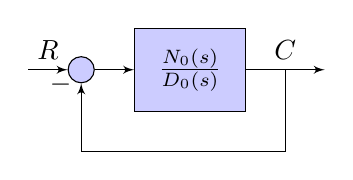
\begin{tikzpicture}[auto, >=latex']
% Nodes
\node [input] (input) {};
\node [sum, right = 0.5cm of input] (sum) {};
\node [block, right = 0.5cm of sum] (system) {$\frac{N_0(s)}{D_0(s)}$};
\node [output, right = 1cm of system] (output) {};
\node [input, below = 0.5cm of system] (m) {};
% Arrows
\draw [draw,->] (input) -- node {$R$} (sum);
\draw [->] (sum) -- node {} (system);
\draw [->] (system) -- node (y) {$C$}(output);
\draw [-] (y) |- (m) {} ;
\draw [->] (m) -| node[pos=0.99] {$-$}  node [near end] {} (sum);
\end{tikzpicture}  
\hspace{0.5cm}
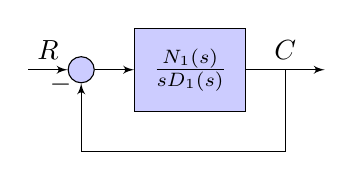
\begin{tikzpicture}[auto, >=latex']
% Nodes
\node [input] (input) {};
\node [sum, right = 0.5cm of input] (sum) {};
\node [block, right = 0.5cm of sum] (system) {$\frac{N_1(s)}{sD_1(s)}$};
\node [output, right = 1cm of system] (output) {};
\node [input, below = 0.5cm of system] (m) {};
% Arrows
\draw [draw,->] (input) -- node {$R$} (sum);
\draw [->] (sum) -- node {} (system);
\draw [->] (system) -- node (y) {$C$}(output);
\draw [-] (y) |- (m) {} ;
\draw [->] (m) -| node[pos=0.99] {$-$}  node [near end] {} (sum);
\end{tikzpicture}  
\hspace{0.5cm}
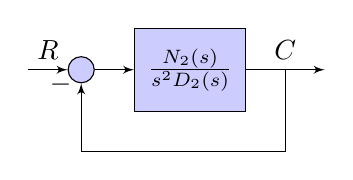
\begin{tikzpicture}[auto, >=latex']
% Nodes
\node [input] (input) {};
\node [sum, right = 0.5cm of input] (sum) {};
\node [block, right = 0.5cm of sum] (system) {$\frac{N_2(s)}{s^2D_2(s)}$};
\node [output, right = 1cm of system] (output) {};
\node [input, below = 0.5cm of system] (m) {};
% Arrows
\draw [draw,->] (input) -- node {$R$} (sum);
\draw [->] (sum) -- node {} (system);
\draw [->] (system) -- node (y) {$C$}(output);
\draw [-] (y) |- (m) {} ;
\draw [->] (m) -| node[pos=0.99] {$-$}  node [near end] {} (sum);
\end{tikzpicture}  
\caption{Systems of types 0, 1 and 2. Note that $N_0, N_1, N_2, D_0,
	D_1, D_2$ should not be factorizable by $s$.}
\end{figure}
\end{document}